\documentclass[
11pt, % The default document font size, options: 10pt, 11pt, 12pt
%oneside, % Two side (alternating margins) for binding by default, uncomment to switch to one side
english, % ngerman for German
%singlespacing, % Single line spacing, alternatives: onehalfspacing or doublespacing
%onehalfspacing, % Single line spacing, alternatives: onehalfspacing or doublespacing
doublespacing, % Single line spacing, alternatives: onehalfspacing or doublespacing
%draft, % Uncomment to enable draft mode (no pictures, no links, overfull hboxes indicated)
%nolistspacing, % If the document is onehalfspacing or doublespacing, uncomment this to set spacing in lists to single
liststotoc, % Uncomment to add the list of figures/tables/etc to the table of contents
%toctotoc, % Uncomment to add the main table of contents to the table of contents
%parskip, % Uncomment to add space between paragraphs
%nohyperref, % Uncomment to not load the hyperref package
headsepline, % Uncomment to get a line under the header
%chapterinoneline, % Uncomment to place the chapter title next to the number on one line
%consistentlayout, % Uncomment to change the layout of the declaration, abstract and acknowledgements pages to match the default layout
]{MastersDoctoralThesis} % The class file specifying the document structure

\usepackage[utf8]{inputenc} % Required for inputting international characters
\usepackage[T1]{fontenc} % Output font encoding for international characters
\usepackage{mathpazo} % Use the Palatino font by default
\usepackage{amsthm}
\usepackage{amsmath,amssymb,amsfonts}
\usepackage[autostyle=true]{csquotes} % Required to generate language-dependent quotes in the bibliography
\usepackage{graphicx} 
\usepackage{layout}
\usepackage{multicol}
\usepackage{multirow}
\usepackage{caption}
\usepackage{subcaption}
\usepackage[final]{hyperref}
%\usepackage{cleveref}
%\usepackage{titlesec}
\usepackage{cite}
\usepackage{siunitx}
\usepackage{hyphenat}
\usepackage{notoccite}
\usepackage{CJKutf8}
\usepackage{dashrule}

%----------------------------------------------------------------------------------------
%	Table Setting
%----------------------------------------------------------------------------------------
\usepackage{booktabs}% http://ctan.org/pkg/booktabs
\newcommand{\tabitem}{~~\llap{\textbullet}~~}

%
%----------------------------------------------------------------------------------------
%	MARGIN SETTINGS
%----------------------------------------------------------------------------------------

\geometry{
	paper=a4paper, % Change to letterpaper for US letter
%	inner=2.5cm, % Inner margin
%	outer=3.8cm, % Outer margin
%	bindingoffset=.5cm, % Binding offset
	top=5.7cm, % Top margin
	bottom=4.2cm, % Bottom margin
	left=2.5cm, % Left margin
	right=5cm, % Right margin
%	showframe, % Uncomment to show how the type block is set on the page
}

%----------------------------------------------------------------------------------------
%	HEADER SETTINGS
%----------------------------------------------------------------------------------------

%\titleformat{\chapter}[display]
%{\bfseries\LARGE}
%{\filcenter\Large\chaptertitlename~\thechapter}
%{1ex}
%{\titlerule\vspace{1.5ex}\filright}
%[\vspace{1ex}\titlerule]

%----------------------------------------------------------------------------------------
%	CUSTOM COMMANDS
%----------------------------------------------------------------------------------------

% Set counter for subsubsections
\setcounter{tocdepth}{2}
\setcounter{secnumdepth}{3}

% Definitions counter
\newcounter{definition}[chapter]
\renewcommand\thedefinition{\thechapter.\arabic{definition}}
\newcommand\definitionname{Definition}
\newenvironment{definition}[1][]
{\refstepcounter{definition}
	\par\medskip
	\noindent \textbf{\definitionname~\thedefinition. #1}
	\rmfamily}{\medskip}


%----------------------------------------------------------------------------------------
%	THESIS INFORMATION
%----------------------------------------------------------------------------------------

\thesistitle{Your Title} % Your thesis title, this is used in the title and abstract, print it elsewhere with \ttitle
\supervisor{Prof. Jin Woo \textsc{Song}} % Your supervisor's name, this is used in the title page, print it elsewhere with \supname
%\examiner{} % Your examiner's name, this is not currently used anywhere in the template, print it elsewhere with \examname
\degree{Master of Engineering} % Your degree name, this is used in the title page and abstract, print it elsewhere with \degreename
\author{Your Name} % Your name, this is used in the title page and abstract, print it elsewhere with \authorname
%\addresses{} % Your address, this is not currently used anywhere in the template, print it elsewhere with \addressname

\subject{Intelligent Mechatronics Engineering} % Your subject area, this is not currently used anywhere in the template, print it elsewhere with \subjectname
\keywords{} % Keywords for your thesis, this is not currently used anywhere in the template, print it elsewhere with \keywordnames
\university{\href{https://eng.sejong.ac.kr/}{Sejong University}} % Your university's name and URL, this is used in the title page and abstract, print it elsewhere with \univname
\department{\href{https://eng.sejong.ac.kr/contents/eng/cor/engineering_6.html}{Department of Intelligent Mechatronics Engineering}} % Your department's name and URL, this is used in the title page and abstract, print it elsewhere with \deptname
\group{\href{https://sites.google.com/view/incsl}{intelligent Navigation and Control Systems Laboratory }} % Your research group's name and URL, this is used in the title page, print it elsewhere with \groupname
\faculty{\href{https://eng.sejong.ac.kr/contents/eng/cor/engineering_6.html}{Faculty of Software Convergence}} % Your faculty's name and URL, this is used in the title page and abstract, print it elsewhere with \facname

\AtBeginDocument{
	\hypersetup{pdftitle=\ttitle} % Set the PDF's title to your title
	\hypersetup{pdfauthor=\authorname} % Set the PDF's author to your name
	\hypersetup{pdfkeywords=\keywordnames} % Set the PDF's keywords to your keywords
	\hypersetup{hidelinks}
}

\begin{document}
	
	\frontmatter % Use roman page numbering style (i, ii, iii, iv...) for the pre-content pages
	
	\pagestyle{plain} % Default to the plain heading style until the thesis style is called for the body content
	
%----------------------------------------------------------------------------------------
%	TITLE PAGE 1
%----------------------------------------------------------------------------------------

\begin{titlepage}
	\begin{center}
		
		\vspace*{.01\textheight}
		
		{\bfseries \fontsize{21}{20}\selectfont \ttitle\par}\vspace{3cm} 
		
		{\fontsize{16}{12}\selectfont \authorname\par}\vspace{2.5cm} 
		
		{\fontsize{14}{12}\selectfont February 2021\par}\vspace{2.5cm} 
		
		{\fontsize{16}{12}\selectfont  \deptname\par}\vspace{0.4cm}
		{\fontsize{16}{12}\selectfont  Department of Convergence Engineering for Intelligent Drone\par}\vspace{0.4cm}
		{\fontsize{16}{12}\selectfont  The Graduate School\par}\vspace{0.4cm} 
		{\fontsize{16}{12}\selectfont  \univname \par}
		
		\vfill
	\end{center}
\end{titlepage}


%----------------------------------------------------------------------------------------
%	TITLE PAGE 2
%----------------------------------------------------------------------------------------

\begin{titlepage}
	\begin{center}
		
		\vspace*{.01\textheight}
		
		{\bfseries \fontsize{21}{20}\selectfont \ttitle\par}\vspace{3cm} 
		
		{\fontsize{16}{12}\selectfont \authorname\par}\vspace{2cm} 
		
		{\fontsize{14}{12}\selectfont A thesis submitted to the Faculty of the Sejong University in partial fulfillment of the requirements for the dual degree of Master in Intelligent Mechatronics Engineering and Master in Convergence Engineering for Intelligent Drone\par}\vspace{2cm} 
		
		{\fontsize{14}{12}\selectfont February 2021\par}\vspace{2cm} 
		
		{\fontsize{14}{12}\selectfont Approved by Major Advisor \par
			Professor Jin Woo Song}\vspace{2cm} 
		
		\vfill
	\end{center}
\end{titlepage}


%----------------------------------------------------------------------------------------
%	TITLE PAGE 3
%----------------------------------------------------------------------------------------

\begin{titlepage}
	\begin{center}
		
		\vspace*{.01\textheight}
		
		{\bfseries \fontsize{16}{20}\selectfont \ttitle\par}\vspace{2cm} 
		
		{\fontsize{11}{11}\selectfont by\par}\vspace{0.2cm} 
		
		{\fontsize{14}{12}\selectfont \authorname\par}\vspace{2cm} 
		
		{\fontsize{14}{1}\selectfont Approved 
			\fontsize{10}{1}\selectfont
			{$-----------------------$}
			\\ 
			\begin{flushleft}
				\hspace{3.8cm}
				\fontsize{12}{11}\selectfont
				..., Chair of the committee
			\end{flushleft}
			}\vspace{1.6cm} 

		{\fontsize{14}{1}\selectfont Approved 
		\fontsize{10}{1}\selectfont
		{$-----------------------$}
		\\
		\begin{flushleft}
			\hspace{3.8cm}
			\fontsize{12}{11}\selectfont
			..., Member of master committee
		\end{flushleft}
		}\vspace{1.6cm} 

		{\fontsize{14}{1}\selectfont Approved 
		\fontsize{10}{1}\selectfont
		{$-----------------------$}
		\\
		\begin{flushleft}
			\hspace{3.8cm}
			\fontsize{12}{11}\selectfont
			Jin Woo Song, Advisor
		\end{flushleft}   
		}\vspace{1.6cm} 
		
		\vfill
	\end{center}
\end{titlepage}
	
	%----------------------------------------------------------------------------------------
	%	QUOTATION PAGE
	%----------------------------------------------------------------------------------------
	
	\vspace*{0.2\textheight}
	
	\noindent\enquote{\itshape Your quotation.}\bigbreak
	
	\hfill ...
	
	%----------------------------------------------------------------------------------------
	%	ABSTRACT PAGE
	%----------------------------------------------------------------------------------------

	\begin{abstract}
		\addchaptertocentry{\abstractname} % Add the abstract to the table of contents
		%----------------------------------------------------------------------------------------
		Your abstract...
		\\
		\\		
		{\bf Keywords: } Your keyword,...
	\end{abstract}
%	

	%----------------------------------------------------------------------------------------
	%	LIST OF CONTENTS/FIGURES/TABLES PAGES
	%----------------------------------------------------------------------------------------

	\setcounter{tocdepth}{1}
	\tableofcontents % Prints the main table of contents
	
	\listoffigures % Prints the list of figures
	
	\listoftables % Prints the list of tables
	
	%----------------------------------------------------------------------------------------
	%	ABBREVIATIONS
	%----------------------------------------------------------------------------------------
	
	 \begin{abbreviations}{l|l} % Include a list of abbreviations (a table of two columns)
	%
	 \textbf{i.e.} & \text{In Other Words} \\
	 \textbf{e.g.} & \text{For Example} \\
	 \textbf{etc.} & \text{Et Cetera}
	 \end{abbreviations}
	
	%----------------------------------------------------------------------------------------
	%	THESIS CONTENT - CHAPTERS
	%----------------------------------------------------------------------------------------
	
	\mainmatter % Begin numeric (1,2,3...) page numbering
	
	\pagestyle{thesis} % Return the page headers back to the "thesis" style
	
	\chapter{Introduction} 

\label{Introduction}

%----------------------------------------------------------------------------------------
% 											Section 1
\section{Section 1}
Your section content...

You can start your citation here, for example, "in the book \cite{titterton2004strapdown}
\subsection{Sub-section 1}
Your sub-section content...

Example of one figure in one line (Fig. \ref{drone_fig_1})

\begin{figure}
	\centering
	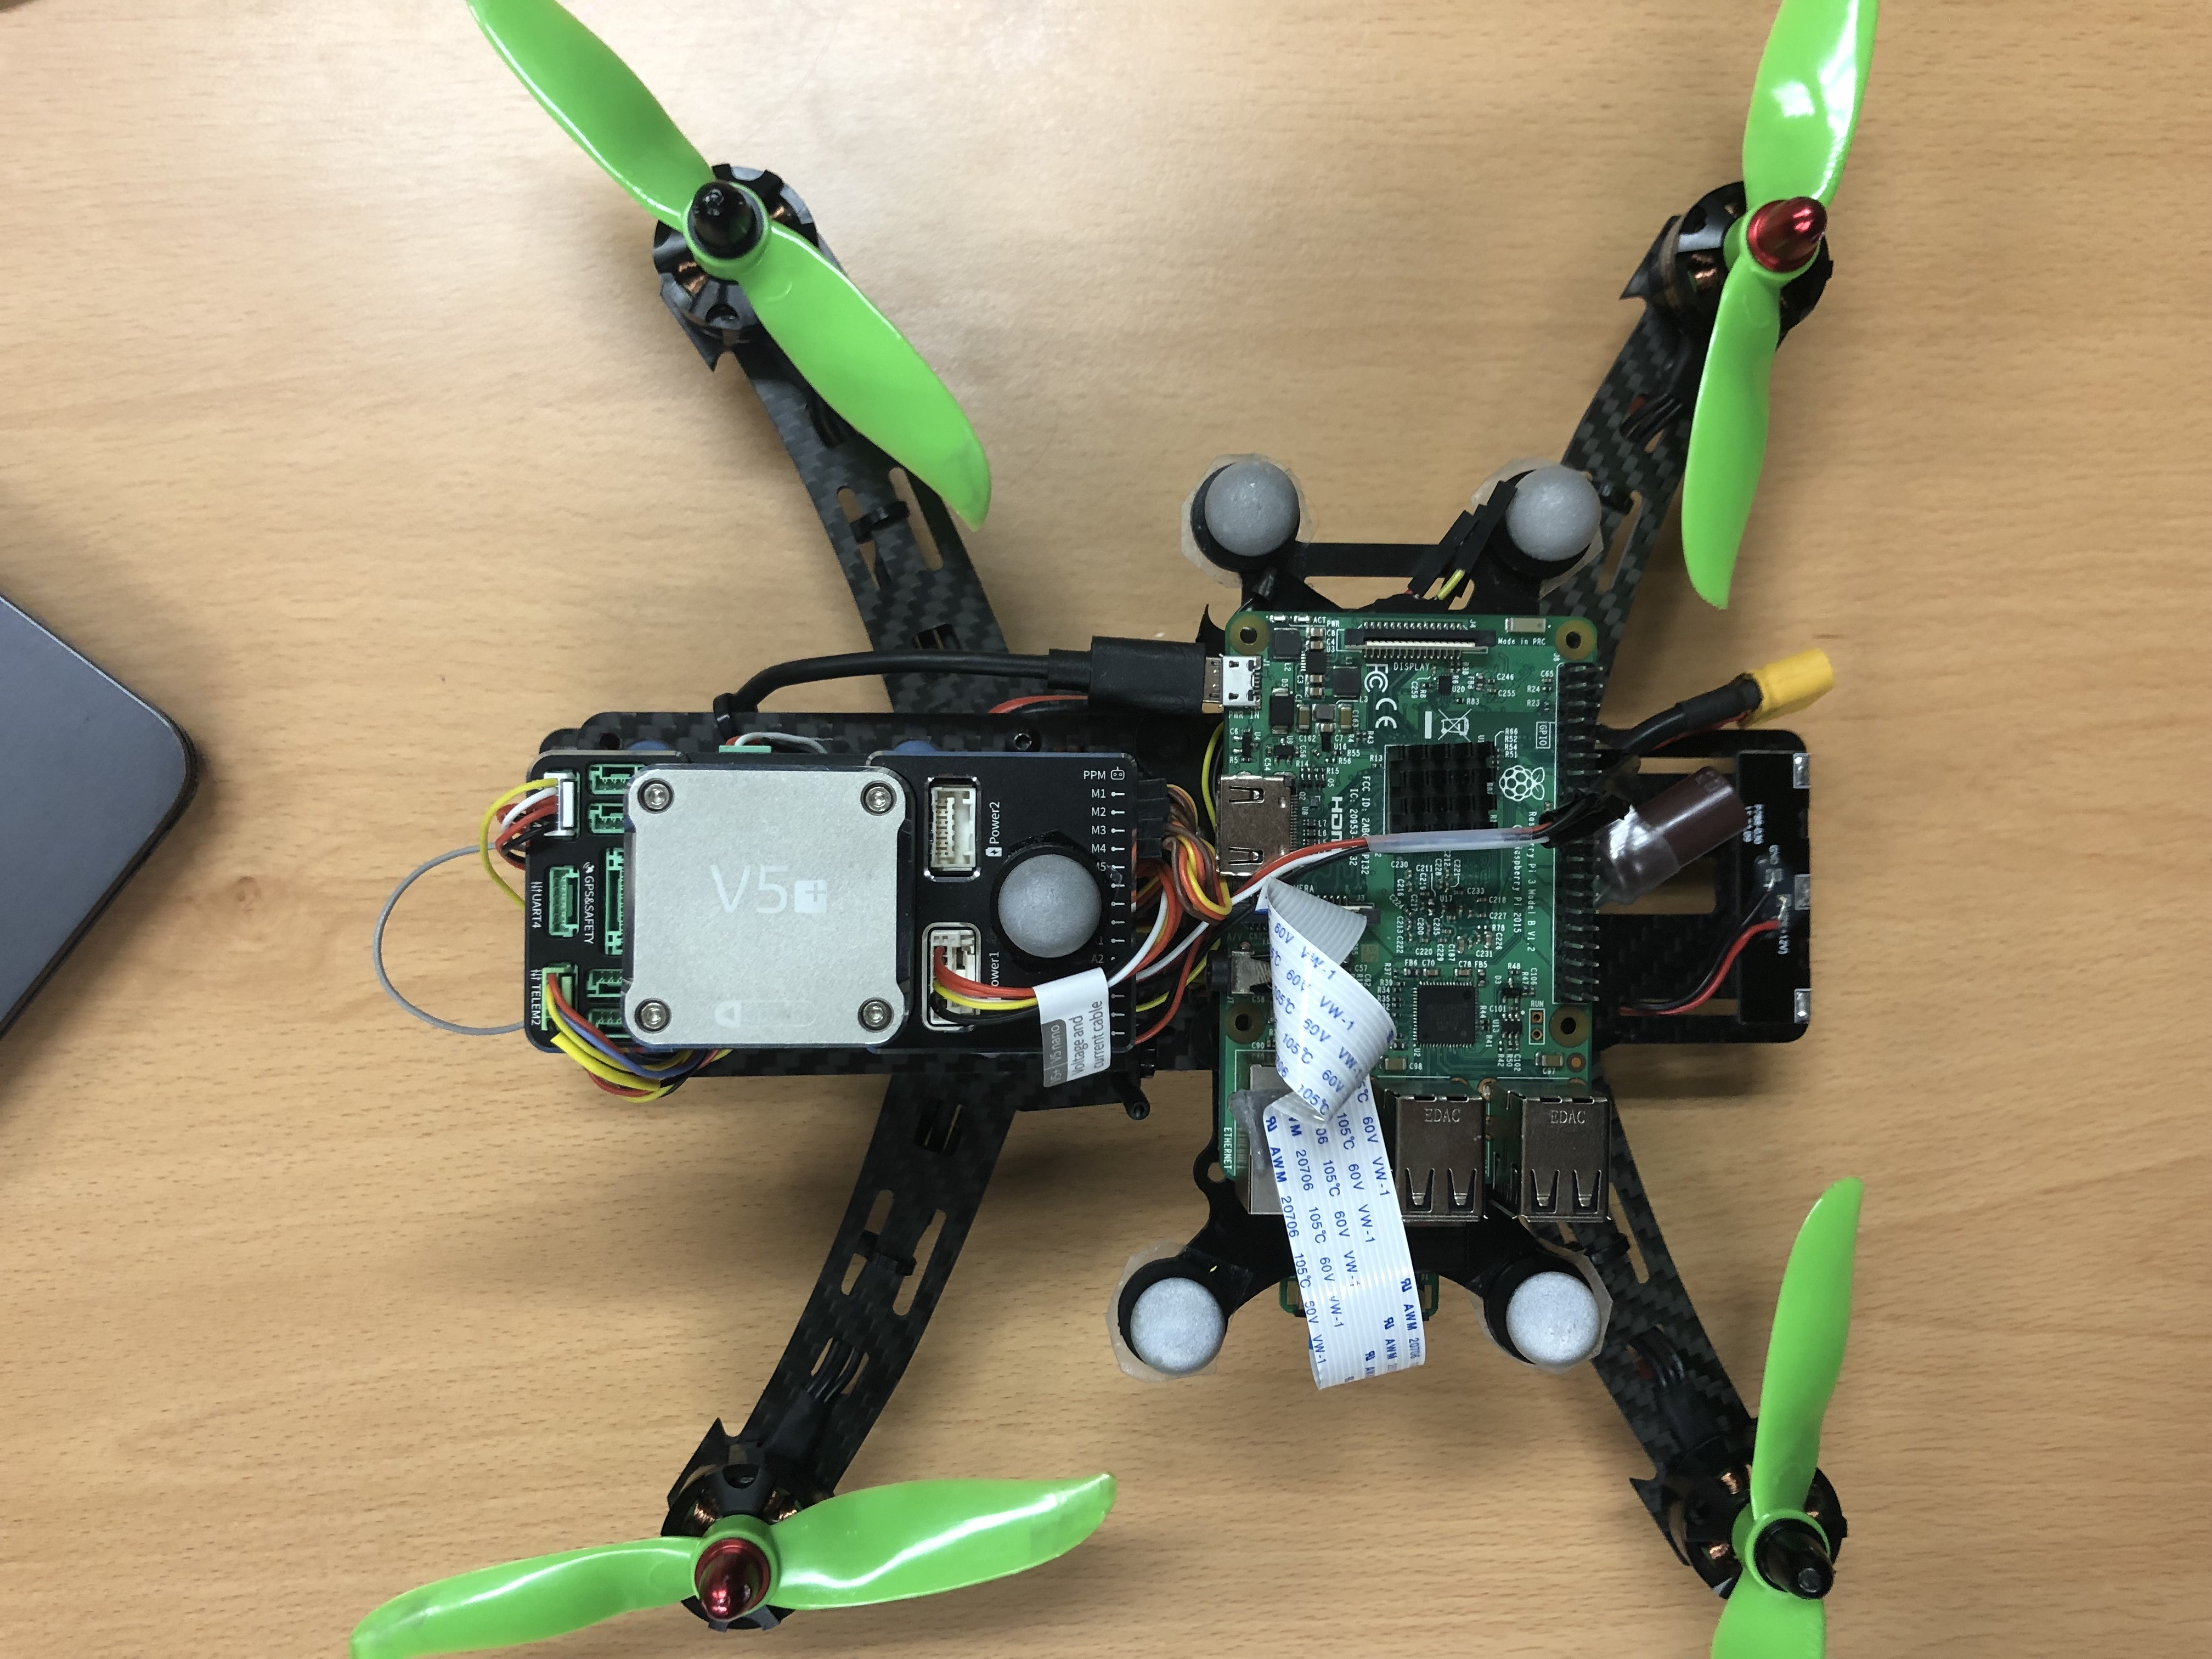
\includegraphics[width=\textwidth,keepaspectratio]{Figures/drone_setup.jpg}
	\caption{caption}
	\label{drone_fig_1}
\end{figure}
	

Example of two figures in one line (Fig. \ref{drone_fig_2})
\begin{figure}
	\centering
	\begin{subfigure}[b]{0.49\textwidth}
		\centering
		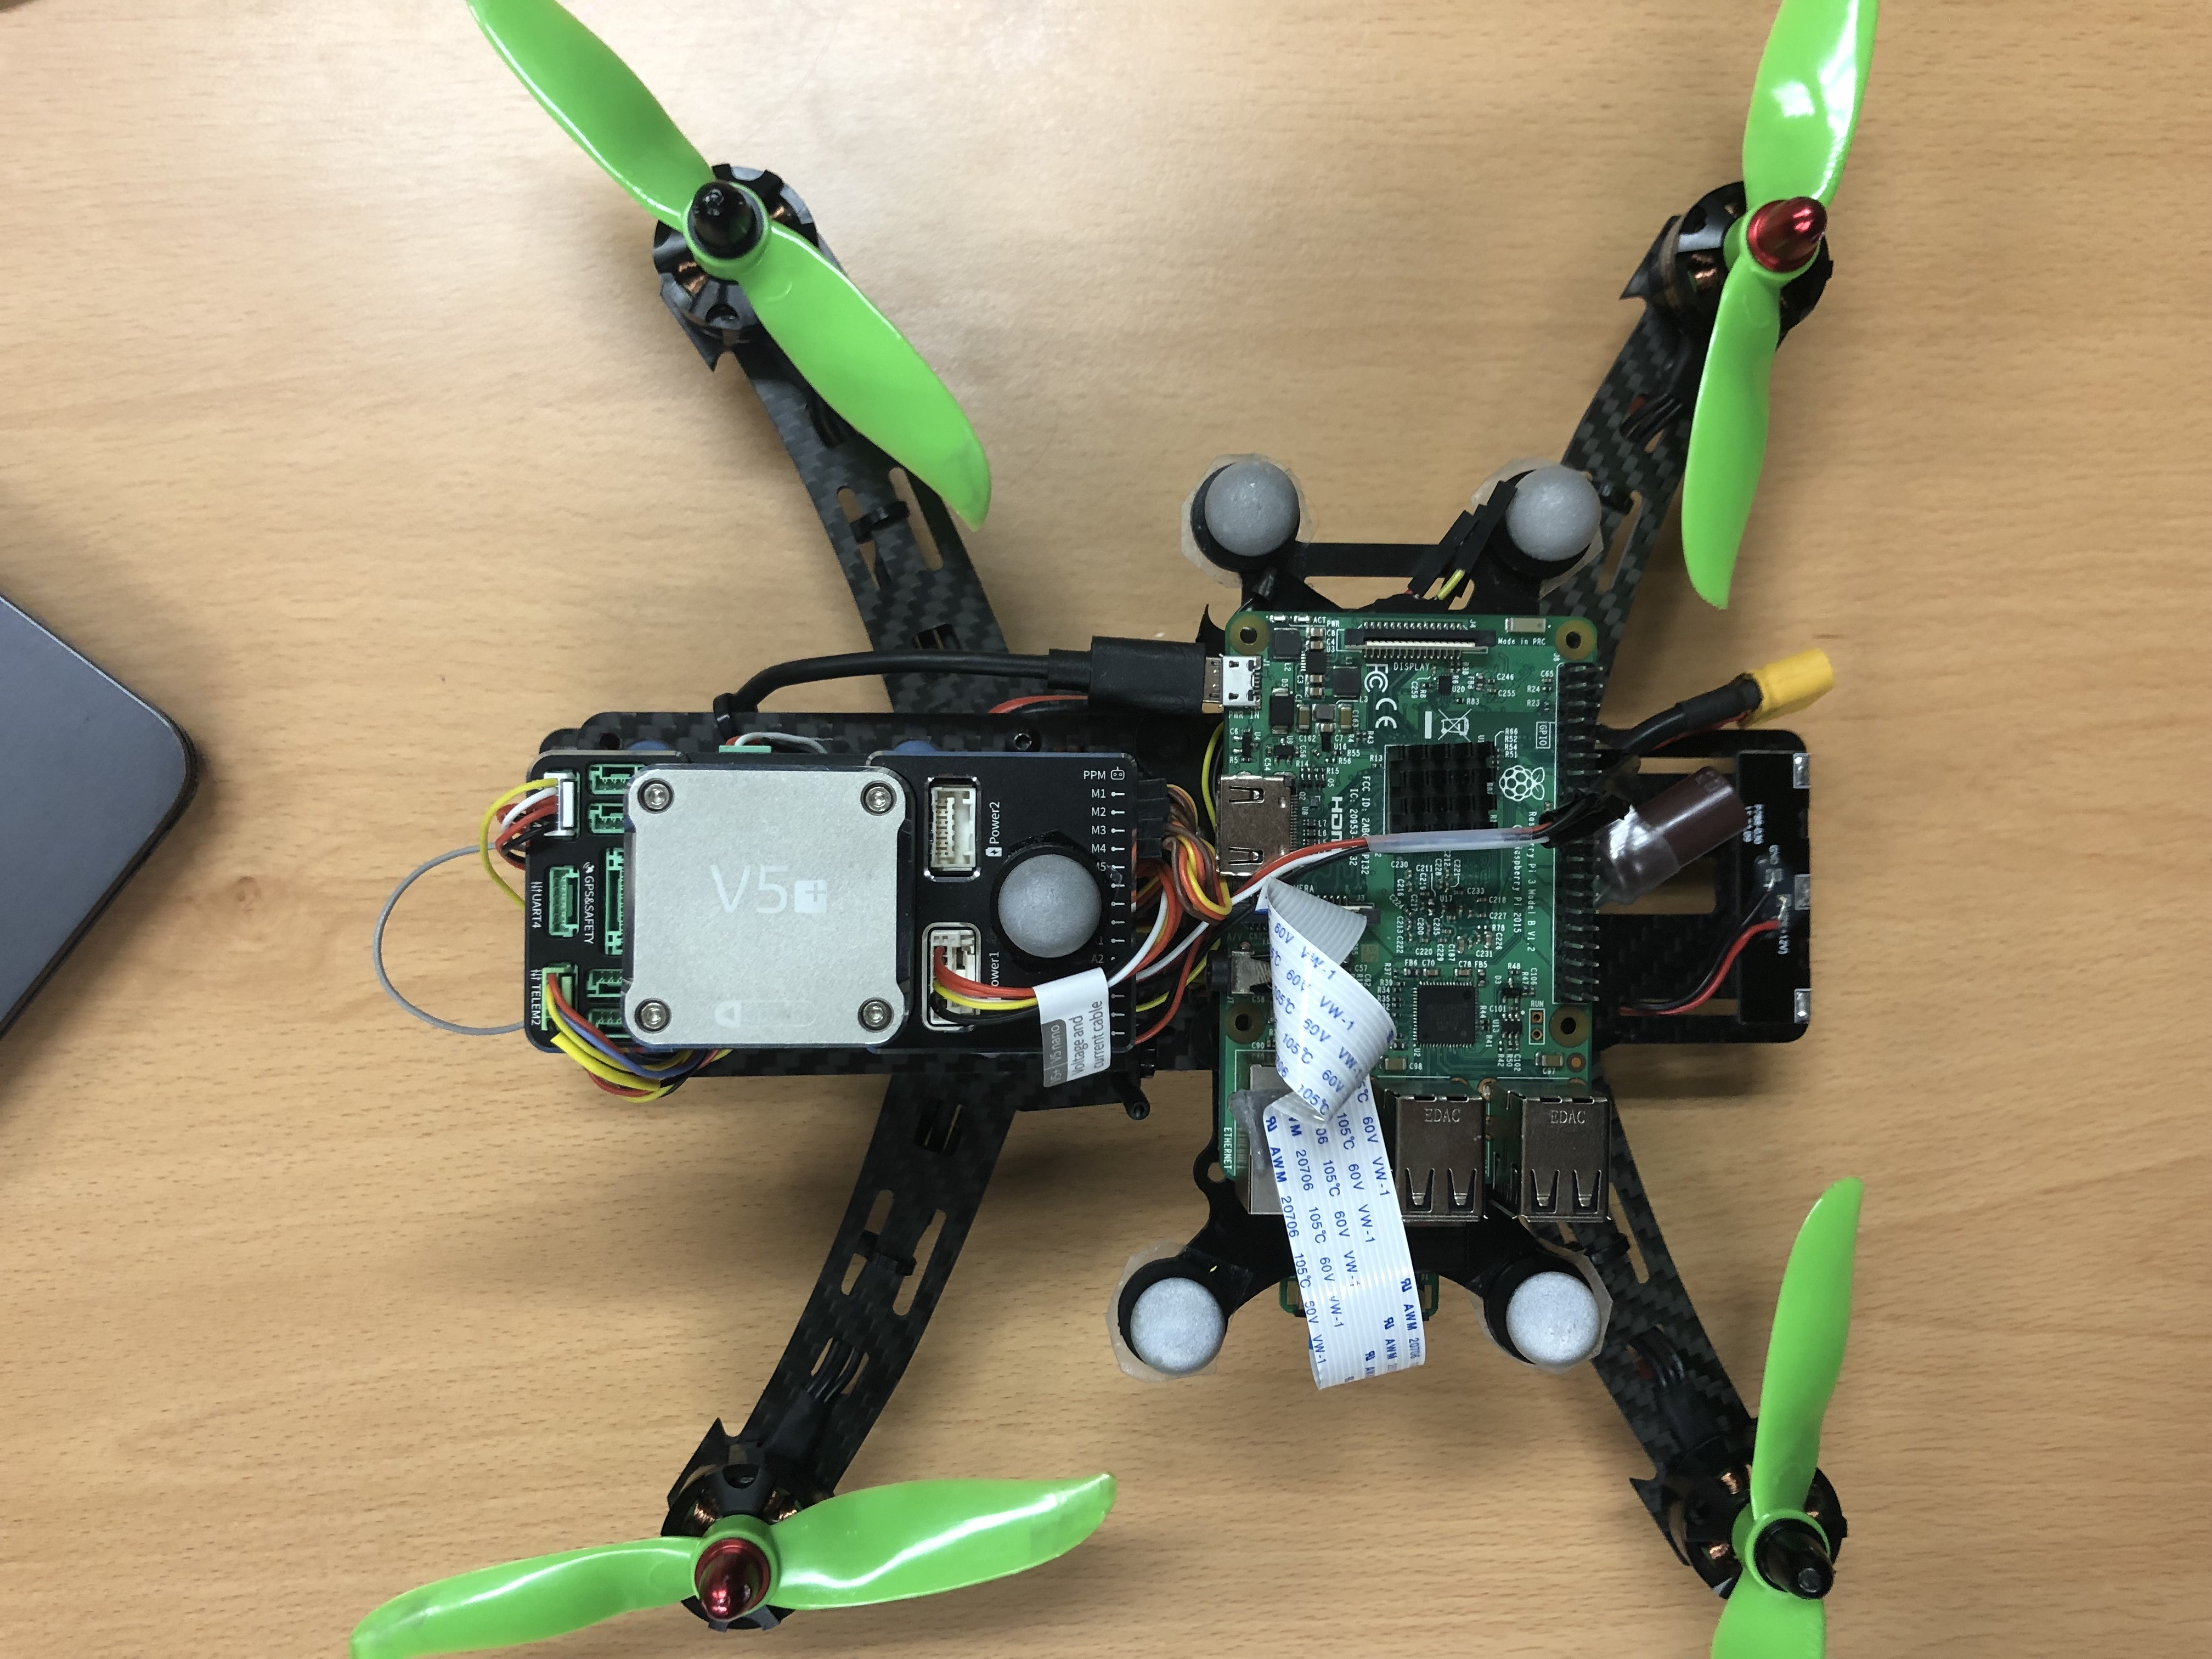
\includegraphics[width=\textwidth,keepaspectratio]{Figures/drone_setup.jpg}
	\end{subfigure}
	\begin{subfigure}[b]{0.49\textwidth}
		\centering
		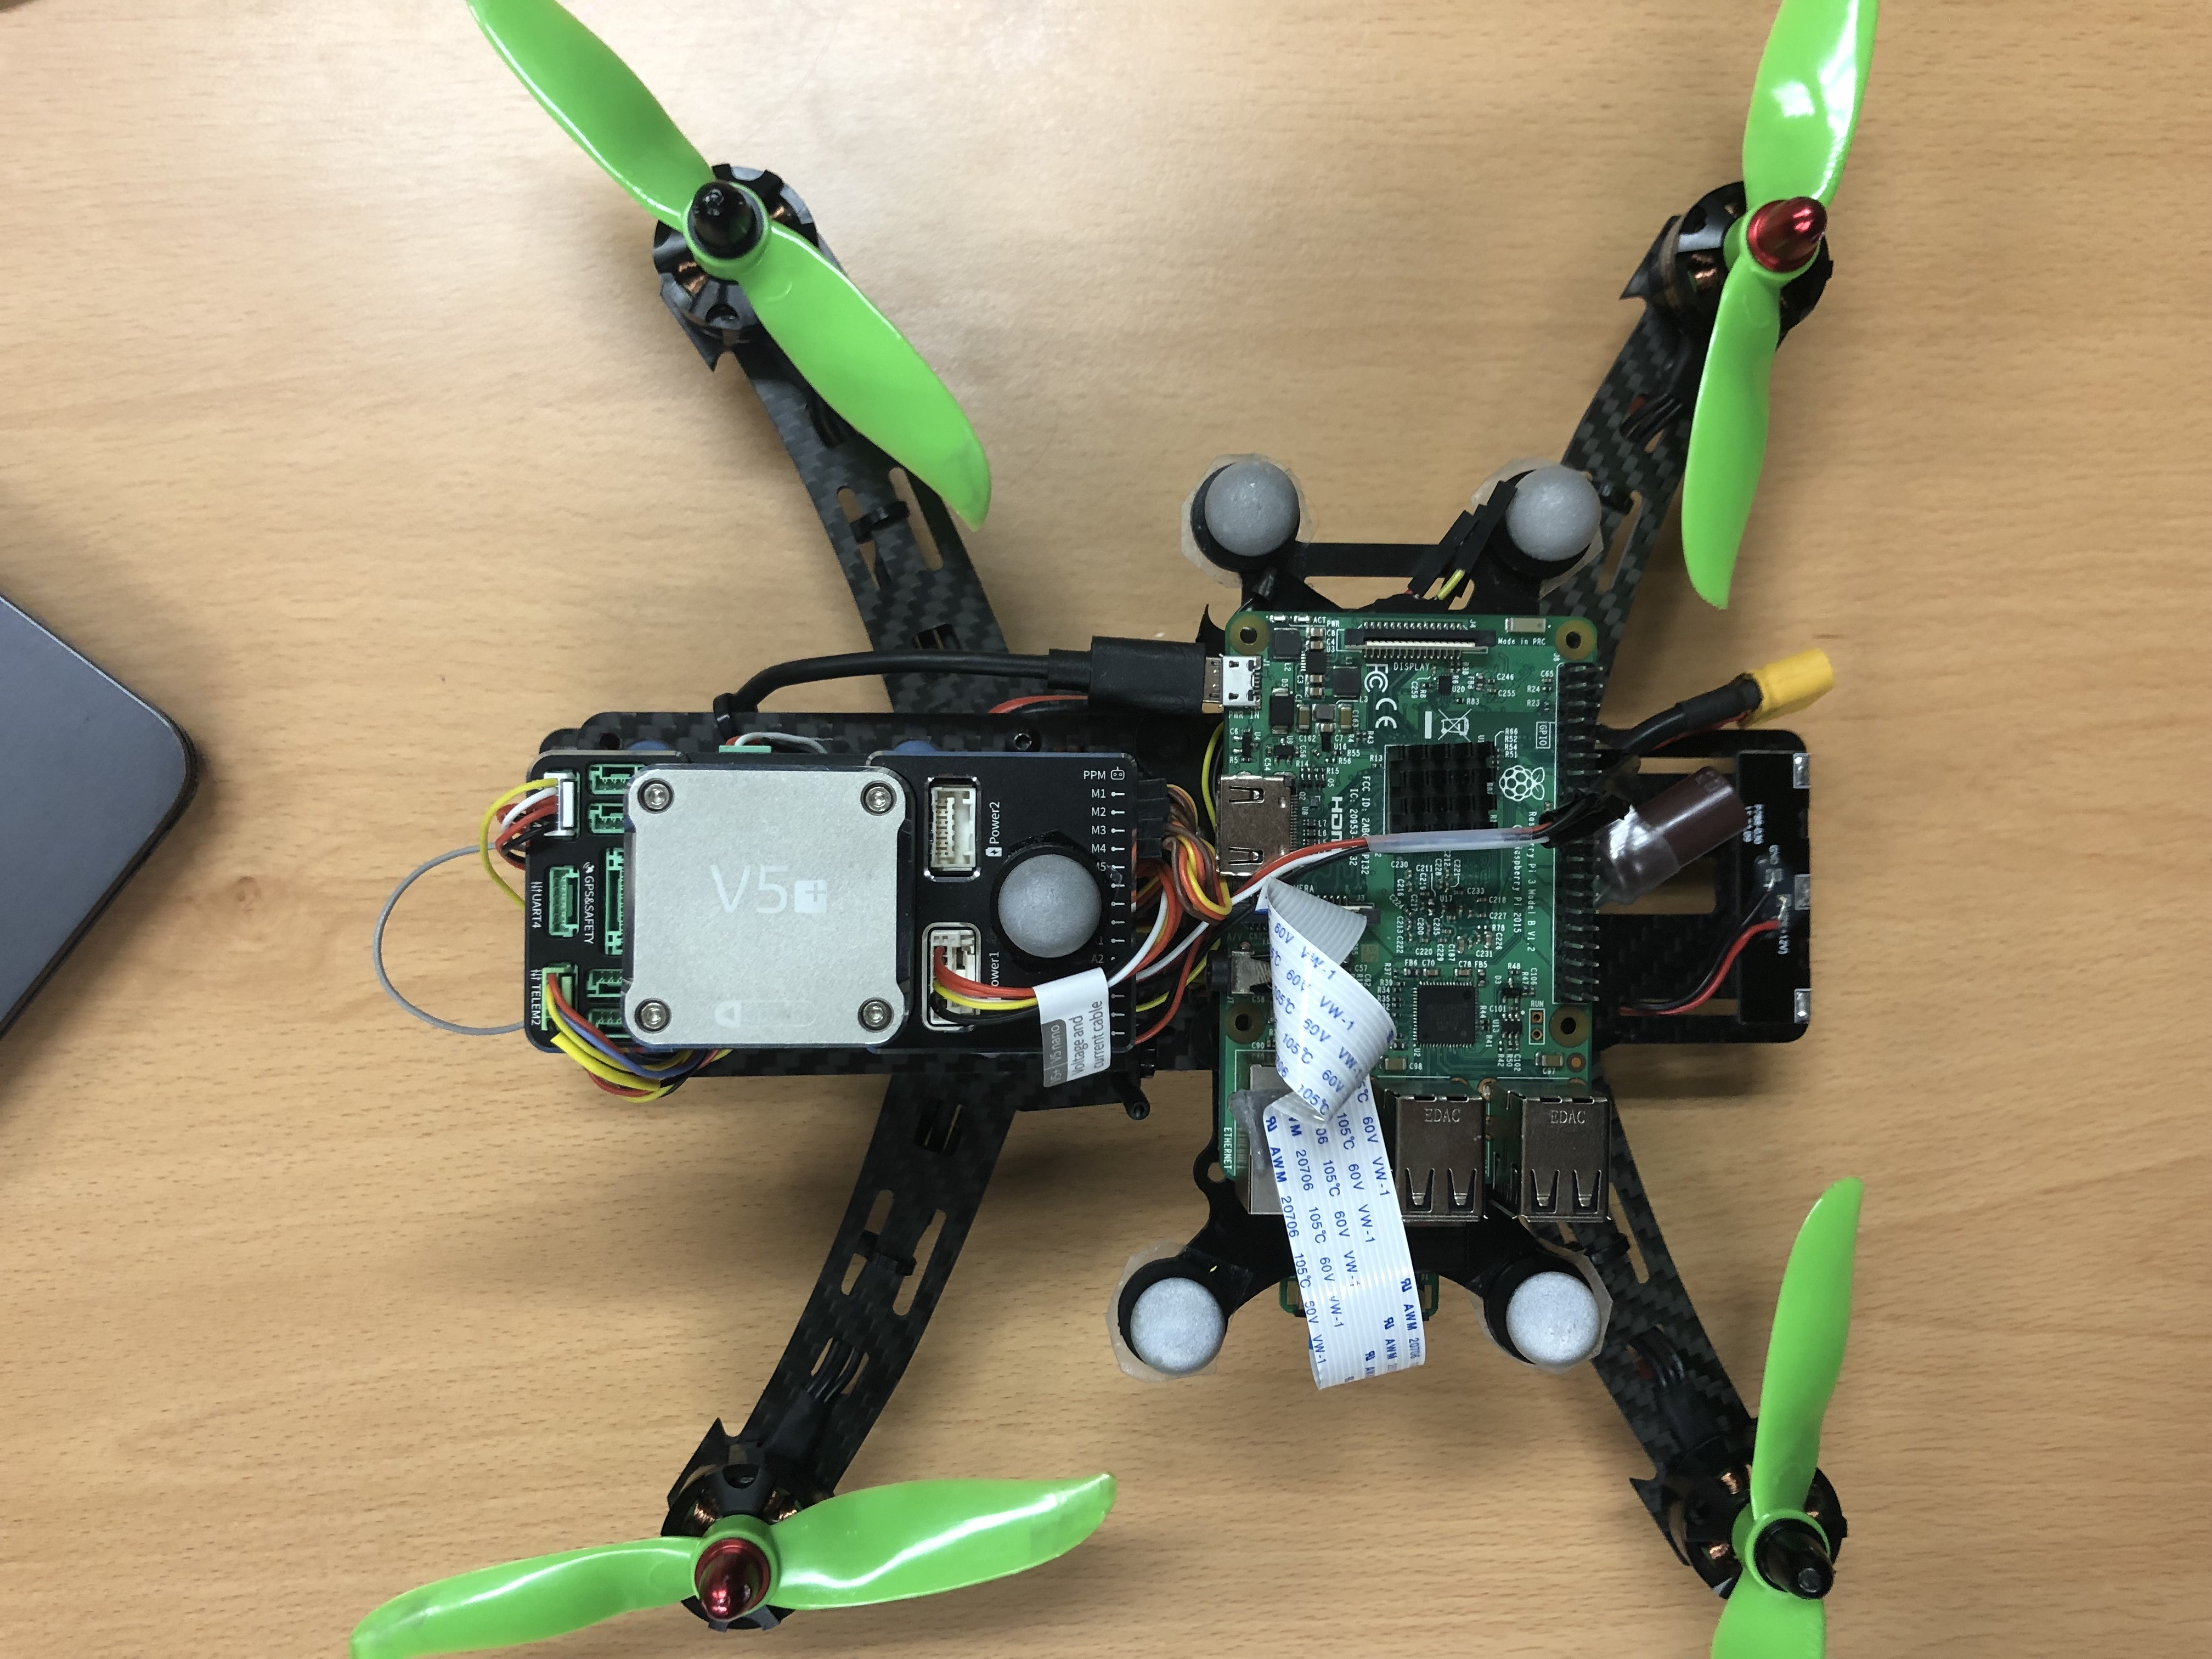
\includegraphics[width=\textwidth,keepaspectratio]{Figures/drone_setup.jpg}
	\end{subfigure}
	\caption{caption}
	\label{drone_fig_2}
\end{figure}

Example of Table \ref{sensors_table}

\begin{table}[ht]
	\centering
	\setlength{\tabcolsep}{4pt} % Default value: 6pt
	\renewcommand{\arraystretch}{1.5} % Default value: 1
	\begin{tabular}{|c|c|c|}
		\toprule
		& \textbf{Measurement} & \textbf{Drawbacks} \\
		\midrule
		IMU & Linear Accelerations, & Biased and noisy measurements, \\
		& Angular velocities.   & Large uncertain for slow motions.\\
		
		\midrule
		GNSS & Absolute position (outdoor). & Unreliable in indoor \\
		&                              & and urban environments. \\
		\midrule
		Magnetic  & Earth's magnetic  & Disturbed by electronic \\
		Sensor    & field direction.  & devices nearby. \\
		\midrule
		Barometric & Absolute altitude. & Not reliable indoor, \\
		&					& Affected by weather conditions. \\
		\midrule							   
		Camera & Inertial measurement, & Ambiguity, calibration, \\
		& Visual information.   & Affected by light conditions. \\
		
		\midrule
		Laser & Distance to objects & Heavy and expensive, \\
		&  					& 2D information. \\
		\bottomrule
	\end{tabular}
	\caption{Properties of some sensors that are commonly used for estimation task in the literature.}
	\label{sensors_table}
\end{table}


	
	%----------------------------------------------------------------------------------------
	%	BIBLIOGRAPHY
	%----------------------------------------------------------------------------------------
	
	\bibliographystyle{IEEEtran}
	\bibliography{IEEEabrv,bibtex}
	
	%----------------------------------------------------------------------------------------

	%----------------------------------------------------------------------------------------
	%	THESIS CONTENT - APPENDICES
	%----------------------------------------------------------------------------------------
	
	\appendix % Cue to tell LaTeX that the following "chapters" are Appendices
	
	% Include the appendices of the thesis as separate files from the Appendices folder
	% Uncomment the lines as you write the Appendices
	
	\include{Appendices/First Appendix}

	%----------------------------------------------------------------------------------------
	% KOREAN	ABSTRACT PAGE
	%----------------------------------------------------------------------------------------
\begin{krabstract}
	\addchaptertocentry{Korean Abstract} % Add the abstract to the table of contents
	\begin{CJK}{UTF8}{}
		\CJKfamily{mj}
		\vspace{1.2cm}
		\begin{center}
			{\fontsize{16}{12}\selectfont 다양한 이동 측정치를 활용한 다중 상태 제약 칼만필터 기반 영상관성 융합 항법 시스템\par}\vspace{1.2cm}
			\begin{flushright}
				{\fontsize{14}{12}\selectfont 세종대학교 일반대학원\par}\vspace{0.6cm} 
				{\fontsize{14}{12}\selectfont 소프트웨어학과\par}\vspace{0.6cm}
				{\fontsize{14}{12}\selectfont 지능형드론 융합전공\par}\vspace{0.6cm}
				{\fontsize{14}{12}\selectfont Your name\par}
			\end{flushright}
		\end{center}
		\vspace{2cm} 
		Your abstract in Korean

		{\bf 키워드:} Your keyword in Korean.
	\end{CJK}	
\end{krabstract}

	%----------------------------------------------------------------------------------------
	%	ACKNOWLEDGEMENTS
	%----------------------------------------------------------------------------------------
	\begin{acknowledgements}
		\addchaptertocentry{\acknowledgementname} % Add the acknowledgements to the table of contents
		\vspace{1em}
		Your acknowledgements.
	\end{acknowledgements}
\end{document}  